\section{Auswertung}

Für die Rechnungen der Auswertung wird das Programm 
\emph{Python} mit dem Packet \emph{numpy} verwendet. Zur Berechnung
des Mittelwertes der Absorptionskoeffizienten wird die automatische Fehlerrechnung mit
dem Packet \emph{uncertainties} durchgeführt. In den Abschnitten, in denen die
Fehler per Hand mithilfe der Gauß'schen Fehlerfortpflanzung (\ref{eqn:Gauß})
berechnet werden, ist die verwendete Fehlerformel mit angegeben.

\begin{equation}
  \sigma\ua{y} = \sqrt{ \sum_{i} \left(\frac{\partial y}{\partial x_i} \cdot \sigma x_i\right)^2 }
  \label{eqn:Gauß}
\end{equation}

Für die Auswertung werden bei den einzelnen Messungen nur die Counts in einem
bestimmten Intervall verwendet. Die verwendeten Intervalle, sowie die Anzahl
an Counts, deren Fehler und die Messzeit sind in Kapitel \ref{subsec:Absorption}
in den Tabellen \ref{tab:Luft} bis \ref{tab:Unbekannt} dargestellt. Die Messdaten sind Poissonverteilt,
weshalb als Fehler immer die Wurzel der Anzahl der Count verwendet wird.

\subsection{Spektrum von \ce{^{137}Cs}}

In Abbildung \ref{fig:Spektrum} ist das aufgenommene Spektrum bei der Messung
der Projektion $I_6$ des mit Luft gefüllten Würfels dargestellt.

Der Anfangsbereich, in dem keine Zählrate angezeigt wird, entsteht durch den
vorgeschlossenen Diskriminator. Dadurch werden erst Stromstärken über einem
gewissen Schwellenwert registriert, wodurch auch bei Aufnahme des Spektrums
unter einem gewissen Energiewert keine im Szintillator ausgelösten Lichtblitze
registriert werden. Bei dem kleineren Peak handelt es sich um einen Rückstreupeak,
welcher durch die Rückstreuung aufgrund von Compton-Stößen außerhalb des
Szintillators entsteht.

Der flache Bereich ist das Compton-Kontinuum, welches durch die Streuung des
Photons an den Elektronen des Szintillatormaterials entsteht. Dabei wird nicht die
ganze Energie des Photons abgegeben, so dass der Energierest im Szintillator registriert werden kann.
Die abgegebene Energie ist nach der Compton-Formel (\eqref{eqn:Compton}, \cite{Compton})
abhängig vom Streuwinkel. Dies erklärt auch die Kante bzw. den Einbruch der
Zählrate vor dem Photopeak, bei dem ein Streuwinkel von 180° vorhanden ist.

\begin{equation}
  E\ua{C} = E\ua{Ph} - \frac{E\ua{Ph}}{1 + \frac{E\ua{Ph}}{E\ua{c,0}} \cdot (1 - cos(\theta))}
  \label{eqn:Compton}
\end{equation}

Bei dem rechten großen Peak handelt es sich um den Photopeak des
Caesium-Präparates. Hier ist die Energie groß genug um im Szintillatormaterial
zum Photoeffekt zu führen. Dieser Peak bzw. die Intensität wird im Folgenden auch
als Messwert für die Abschirmung bei den verschiedenen Projektionen verwendet.

\begin{figure}[h]
  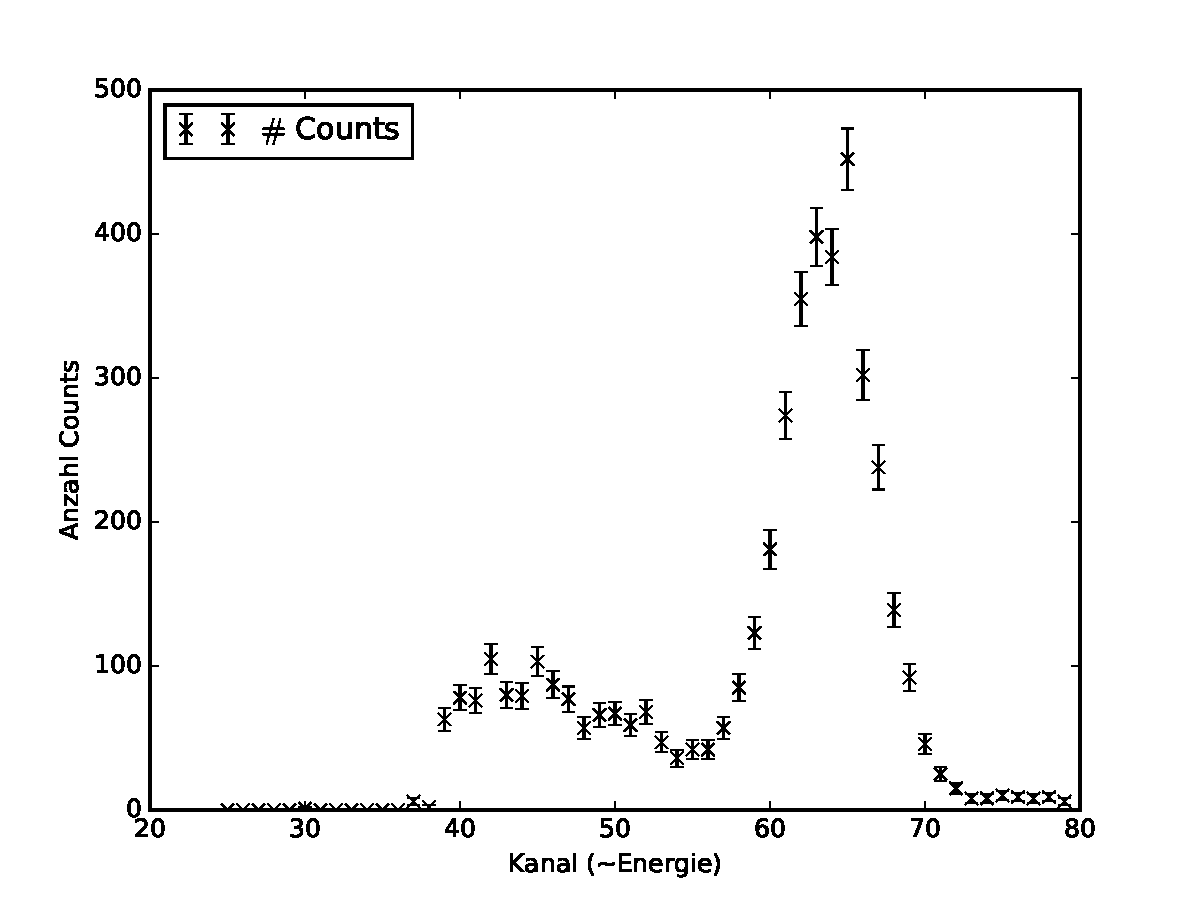
\includegraphics[width = \textwidth]{Daten/Spektrum.pdf}
  \caption{Spektrum der 137 Caesium Quelle bei einem leeren Würfel}
  \label{fig:Spektrum}
\end{figure}

\subsection{Bestimmung der Absorptionskoeffizienten}
\label{subsec:Absorption}

Um die Intensität der einzelnen Projektionen zu bestimmen, werden die gemessenen
Counts bei jeder Projektion mittels der Messzeit normiert. Der Fehler der
Rate ergibt sich dann über Gauß'sche Fehlerfortpflanzung. Die Messzeit wird
hierbei als fehlerfrei angenommen.

\begin{align}
   I\ua{j} &= \frac{N\ua{j}}{T\ua{j}} \\
   \sigma\ua{I\ua{j}} &= \frac{1}{T\ua{j}} \cdot \sigma\ua{N\ua{j}} .
\end{align}

Über die Rate lässt sich dann auch die wie folgt definierte Größe $y$ bestimmen:

\begin{align}
  y\ua{j} &= \su{ln}\left(\frac{I\ua{0}}{I\ua{j}}\right)  \\
  \sigma\ua{y\ua{j}} &= \sqrt{ \left( \frac{\sigma\ua{I}}{I}\right)^2 + \left(\frac{\sigma\ua{I\ua{0}}}{I\ua{0}}\right)^2} .
\end{align}

Der Fehler ergibt sich ebenfalls aus der Gauß'schen Fehlerfortpflanzung. Mit
$I\ua{0}$ ist hierbei die gemessene Rate bei einem leeren Würfel gemeint. Diese
wurde für jede Art von Projektion einmal gemessen ($I\ua{2}$, $I\ua{3}$ und $I\ua{6}$).

\begin{table}
  \centering
  \caption{$I\ua{0}$ für die verschiedenen Projektionen des leeren Würfels.}
  \label{tab:Luft}
  \begin{tabular}{c | c c c c c c}
    \toprule
    Projektion & Kanäle & $T$ in s & $N$ & $\sigma\ua{N}$ & $I$ in $\su{cm}^{-1}$ & $\sigma\ua{I}$ in $\su{cm}^{-1}$ \\
    \midrule
    $I\ua{2}$ & 55-62 & 87 & 16042 & 127 & 184,4 & 1,5 \\
    $I\ua{3}$ & 55-62 & 87 & 16115 & 127 & 185,2 & 1,5 \\
    $I\ua{6}$ & 55-62 & 83 & 15341 & 124 & 184,8 & 1,5 \\
    \bottomrule
  \end{tabular}
\end{table}

\begin{table}
  \centering
  \caption{$I$ für die verschiedenen Projektionen des Aluminiumwürfels.}
  \label{tab:Alu}
  \begin{tabular}{c | c c c c c c c c}
    \toprule
    Projektion & Kanäle & $T$ in s & $N$ & $\sigma\ua{N}$ & $I$ in $\su{cm}^{-1}$
    & $\sigma\ua{I}$ in $\su{cm}^{-1}$ & $y$ & $\sigma\ua{y}$ \\
    \midrule
    $I\ua{1}$  & 63-69 & 84 & 8206 & 91 & 97,7  & 1,1 & 0,64 & 0,01 \\
    $I\ua{2}$  & 62-68 & 30 & 2268 & 48 & 75,6  & 1,6 & 0,89 & 0,02 \\
    $I\ua{3}$  & 61-66 & 26 & 2135 & 46 & 82,1  & 1,8 & 0,81 & 0,02 \\
    $I\ua{4}$  & 59-65 & 26 & 2336 & 48 & 89,9  & 1,9 & 0,72 & 0,02 \\
    $I\ua{5}$  & 59-65 & 30 & 2837 & 53 & 94,6  & 1,8 & 0,67 & 0,02 \\
    $I\ua{6}$  & 59-65 & 24 & 2186 & 47 & 91,1  & 2,0 & 0,71 & 0,02 \\
    $I\ua{7}$  & 59-65 & 24 & 2138 & 47 & 89,1  & 1,9 & 0,73 & 0,02 \\
    $I\ua{8}$  & 59-65 & 29 & 2204 & 47 & 76,0  & 1,6 & 0,89 & 0,02 \\
    $I\ua{9}$  & 58-65 & 34 & 3057 & 55 & 89,9  & 1,6 & 0,72 & 0,02 \\
    $I\ua{10}$ & 58-64 & 26 & 2504 & 50 & 96,3  & 1,9 & 0,65 & 0,02 \\
    $I\ua{11}$ & 58-64 & 24 & 2228 & 47 & 92,8  & 2,0 & 0,69 & 0,02 \\
    $I\ua{12}$ & 57-64 & 23 & 2446 & 50 & 106,3 & 2,2 & 0,55 & 0,02 \\
    \bottomrule
  \end{tabular}
\end{table}

\begin{table}
  \centering
  \caption{$I$ für die verschiedenen Projektionen des Bleiwürfels.}
  \label{tab:Blei}
  \begin{tabular}{c | c c c c c c c c}
    \toprule
    Projektion & Kanäle & $T$ in s & $N$ & $\sigma\ua{N}$ & $I$ in $\su{cm}^{-1}$
    & $\sigma\ua{I}$ in $\su{cm}^{-1}$ & $y$ & $\sigma\ua{y}$ \\
    \midrule
    $I\ua{1}$  & 57-64 & 110 & 1218 & 35 & 11,1 & 0,3 & 2,81 & 0,05 \\
    $I\ua{2}$  & 57-64 & 375 & 1197 & 35 & 3,2  & 0,1 & 4,06 & 0,10 \\
    $I\ua{3}$  & 57-64 & 203 & 1203 & 35 & 5,9  & 0,2 & 3,44 & 0,07 \\
    $I\ua{4}$  & 57-64 & 161 & 1198 & 35 & 7.4  & 0,2 & 3,21 & 0,06 \\
    $I\ua{5}$  & 57-64 & 183 & 1205 & 35 & 6,6  & 0,2 & 3,33 & 0,07 \\
    $I\ua{6}$  & 56-62 & 187 & 1206 & 35 & 6,4  & 0,2 & 3,36 & 0,07 \\
    $I\ua{7}$  & 56-62 & 99  & 1212 & 35 & 12,2 & 0,4 & 2,72 & 0,05 \\
    $I\ua{8}$  & 56-62 & 424 & 1197 & 35 & 2,8  & 0,1 & 4,18 & 0,10 \\
    $I\ua{9}$  & 56-62 & 182 & 1240 & 35 & 6,8  & 0,2 & 3,30 & 0,07 \\
    $I\ua{10}$ & 56-62 & 124 & 1255 & 35 & 10,1 & 0,3 & 2,90 & 0,05 \\
    $I\ua{11}$ & 56-62 & 192 & 1207 & 35 & 6,3  & 0,2 & 3,38 & 0,07 \\
    $I\ua{12}$ & 56-61 & 195 & 1207 & 35 & 6,2  & 0,2 & 3,40 & 0,07 \\
    \bottomrule
  \end{tabular}
\end{table}

\begin{table}
  \centering
  \caption{$I$ für die verschiedenen Projektionen des unbekannten Würfels.}
  \label{tab:Unbekannt}
  \begin{tabular}{c | c c c c c c c c}
    \toprule
    Projektion & Kanäle & $T$ in s & $N$ & $\sigma\ua{N}$ & $I$ in $\su{cm}^{-1}$
    & $\sigma\ua{I}$ in $\su{cm}^{-1}$ & $y$ & $\sigma\ua{y}$ \\
    \midrule
    $I\ua{1}$  & 51-65 & 822  & 12575 & 112 & 15,3  & 0,1 & 2,82 & 0,03 \\
    $I\ua{2}$  & 51-65 & 1503 & 12758 & 113 & 8,5   & 0,1 & 4,06 & 0,03 \\
    $I\ua{3}$  & 51-65 & 690  & 12622 & 112 & 18,3  & 0,2 & 3,44 & 0,02 \\
    $I\ua{4}$  & 52-64 & 648  & 12916 & 114 & 19,9  & 0,2 & 3,21 & 0,02 \\
    $I\ua{5}$  & 52-64 & 700  & 12965 & 114 & 18,5  & 0,2 & 3,33 & 0,02 \\
    $I\ua{6}$  & 52-64 & 683  & 13018 & 114 & 19,1  & 0,2 & 3,36 & 0,02 \\
    $I\ua{7}$  & 52-64 & 341  & 12905 & 114 & 37,8  & 0,3 & 2,72 & 0,02 \\
    $I\ua{8}$  & 52-64 & 1345 & 12840 & 113 & 9,5   & 0,1 & 4,18 & 0,03 \\
    $I\ua{9}$  & 52-64 & 1193 & 12898 & 114 & 10,8  & 0,1 & 3,30 & 0,03 \\
    $I\ua{10}$ & 51-63 & 125  & 12888 & 114 & 103,1 & 0,9 & 2,90 & 0,01 \\
    $I\ua{11}$ & 49-63 & 1407 & 12510 & 112 & 8,9   & 0,1 & 3,38 & 0,03 \\
    $I\ua{12}$ & 49-63 & 799  & 12536 & 112 & 15,7  & 0,1 & 3,40 & 0,03 \\
    \bottomrule
  \end{tabular}
\end{table}


\newpage

Gemäß der Formel \eqref{eqn:kovarianz_I} lässt sich nun die Varianzmatrix $V[\vec{y}]$
bestimmen. Mit ihr wird über Formel \eqref{eqn:kovarianz_mu} die Varianzmatrix
der Absoprtionskoeffizienten bestimmt. Mit den Einträgen auf der Diagonale
lassen sich die Fehler der einzelnen Absorptionskoeffizienten bestimmen.
Zudem werden über Formel \eqref{eqn:mu} die Absorptionskoeffizienten berechnet. Die
Fehler der einzelnen Koeffizienten lassen sich aus den Diagonalelementen von
$V[\vec{\mu}]$ entnehmen:

\begin{equation}
  \sigma\ua{\mu} = \sqrt{V[\vec{\mu}]\ua{ii}}.
\end{equation}

Bei Aluminum und Blei wird mithilfe der automatischen Fehlerrechnung von Python
der Mittelwert der Absorptionskoeffizienten bestimmt. In Tabelle \ref{tab:AluUndBlei}
sind die bestimmten Koeffizienten, deren Fehler sowie die Abweichung zu dem
Literaturwert zu sehen.

\begin{table}
  \centering
  \caption{Bestimmte Absorptionskoeffizienten von Aluminium und Blei und
  die Abweichung zu den Literaturwerten. \cite{Koeffs}}
  \label{tab:AluUndBlei}
  \begin{tabular}{c | c c c c}
    \toprule
    Material & $\mu\ua{exp}$ in $\su{cm}^{-}$ & $\sigma\ua{mu\ua{exp}}$ in
    $\su{cm}^{-}$ & $\mu\ua{lit}$ in $\su{cm}^{-}$ & $\increment \mu$
    in $\su{cm}^{-}$ \\
    \midrule
    Aluminium & 0,227 & 0,003 & 0,202 & 0,0248 $\pm$ 0,003 \\
    Blei      & 1,059 & 0,013 & 1,25  & 0,191 $\pm$ 0,013 \\
    \bottomrule
  \end{tabular}
\end{table}


Für den Würfel unbekannter Zusammensetzung wird gleich Verfahren, um die einzelnen
Absorptionskoeffizienten zu ermitteln. Damit die einzelnen Würfel einem bestimmten Material
zugeordnet werden können,
sind in Tabelle \ref{tab:UnbekanntErgebnis} die Absorptionskoeffizienten, sowie deren
absolute Abweichung
zu den experimentell bestimmten Werten und den Literaturwerten eingetragen. Die Abweichung
wird durch $\increment M$ bezeichnet, wobei $M$ immer der zum Abgleich gezogenen
Koeffizient ist. Die Fehler der Abweichung sind nicht von Interesse und werden
deswegen nicht mit angegeben.

\begin{table}
  \centering
  \caption{Bestimmte Koeffizienten für den unbekannten Würfel sowie die Abweichungen
  zu den anderen Materialien ($|\increment M|$ in $\su{cm}^{-1}$).}
  \label{tab:UnbekanntErgebnis}
  \begin{tabular}{c | c c c c c c c}
    \toprule
    $\mu\ua{i}$ & $\mu$ in $\su{cm}^{-}$ & $\sigma\ua{\mu}$ in $\su{cm}^{-}$ &
    $|\increment \mu\ua{Alu,lit}|$ &
    $|\increment \mu\ua{Alu,exp}|$ &
    $|\increment \mu\ua{Blei,lit}|$ &
    $|\increment \mu\ua{Blei,exp}|$ &
    $\increment\ua{min}$ \\
    \midrule
    $\mu{1}$ & 0,05 & 0,01 & 0,15 & 0,18 & 1,20 & 1,01 & $\mu\ua{Alu}$  \\
    $\mu{2}$ & 1,29 & 0,01 & 1,09 & 1,07 & 0,04 & 0,23 & $\mu\ua{Blei}$ \\
    $\mu{3}$ & 0,82 & 0,02 & 0,61 & 0,59 & 0,43 & 0,24 & $\mu\ua{Blei}$ \\
    $\mu{4}$ & 0,28 & 0,01 & 0,08 & 0,06 & 0,97 & 0,76 & $\mu\ua{Alu}$  \\
    $\mu{5}$ & 1,08 & 0,01 & 0,88 & 0,86 & 0,17 & 0,02 & $\mu\ua{Blei}$ \\
    $\mu{6}$ & 0,92 & 0,01 & 0,62 & 0,59 & 0,43 & 0,24 & $\mu\ua{Blei}$ \\
    $\mu{7}$ & 0,28 & 0,01 & 0,08 & 0,05 & 0,97 & 0,78 & $\mu\ua{Alu}$  \\
    $\mu{8}$ & 0,87 & 0,01 & 0,67 & 0,65 & 0,38 & 0,19 & $\mu\ua{Blei}$ \\
    $\mu{9}$ & 0,96 & 0,02 & 0,76 & 0,74 & 0,29 & 0,10 & $\mu\ua{Blei}$ \\
    \bottomrule
  \end{tabular}
\end{table}


\section{Diskussion}

In Tabelle \ref{tab:UnbekanntErgebnis} ist zu erkennen, dass sich sowohl bei
Vergleich der Koeffizienten mit den experimentell bestimmten Werten, als auch den
Literaturwerten für Aluminium und Blei der gleiche Aufbau für den unbekannten
Würfel ergibt.

Zudem ergab eine Rechnung mit dem Packet \emph{uncertainties} ohne Verwendung der
Varianzmatrizen ähnliche Werte. Lediglich bei sehr geringen Absorptionskoeffizient
ist eine deutliche Abweichung vorhanden, da diese meist in der 2. Nachkommastelle
auftritt.

Obwohl bei der Anzahl $N$ der Counts ein Fehler von $\sqrt{N}$ angenommen wurde, sind
die daraus resultierenden Fehler bei den Absorptionskoeffizienten gering.

Bei der verwendeten Messmethode wurden durch die Mehrfachmessung jedes Würfels
die Absorptionskoeffizienten in Abhängigkeit voneinander bestimmt. Sichtbar ist
dies an der Kovarianzmatrix, in der auch die nicht auf der Hauptdiagonale liegenden
Elemente ungleich Null sind. Diese Abhängigkeit untereinander kann unter anderem
die teilweise starken Abweichungen zu den Literaturwerten erklären.

Eine Fehlerquelle bei diesem Versuch ist unter anderem die Ausdehnung des Strahles,
welcher auch teilweise in benachbarten Blöcken absorbiert wird, wodurch es eine
stärkere Absorption gibt als eigentlich der Fall wäre. Wichtig ist hierbei auch
die Positionierung des Blockes. Bei Messung der Diagonalen ist eine Abweichung
von der theoretischen Projektion nur schwer vermeidbar.

Eine weitere Fehlerquelle ist der umgebende Aluminiumkörper. Zwar wird am Anfang
des Experimentes der Körper vermessen um diese reduzierte Intensiät
als Referenzwert $I\ua{0}$ zu verwenden. Jedoch ist die Dicke des Aluminiummantels
nicht überall gleich, wodurch die Ergebnisse verfälscht werden.
